\section[Direct $C\!P$ asymmetry]
{Direct $\boldsymbol{C\!P}$ asymmetry}
\label{sec:dsphi:acp}

The value of \acp for the decay \btodsphi is calculated using
\begin{equation}
  \acp\big(\btodsphi\big)=
  \frac{N_--N_+}{N_-+N_+-N_\mathrm{bkg}},
  \label{eq:dsphi:acp}
\end{equation}
where $N_-$ and $N_+$ are defined as the signal yields from the charge specific decays \btodsphi
and \decay{\Bm}{\Dsm\phi}, respectively.
The term $N_\mathrm{bkg}$ denotes the amount of background contaminating the signal.

Values of $N_+$, $N_-$ and $N_\mathrm{bkg}$ are determined by defining a signal region, which
extends $\pm2\stdev$ either side of the mean \Bp mass in region \rA, where $\mu=5283\mev$ and
$\sigma=13.2\mev$.
In this region, the number of \Bp and \Bm candidates are $N_+=3$ and $N_-=3$.
The background prediction is determined by integrating across this region, which results in
$N_\mathrm{bkg}=0.75$.
From these values,
$\acp^\mathrm{raw}\big(\btodsphi\big)=\big(0.0\pm0.41\big)$,
where the coverage was obtained using the Feldman-Cousins method~\cite{PhysRevD.57.3873};
which gives a $1\stdev$ interval of $\in[-0.41, 0.41]$.
Figure~\ref{fig:dsphi:aCp} shows the Feldman-Cousins intervals for the \CP asymmetry when observing
six signal events with a background expectation of 0.75.

\begin{figure}
  \begin{center}
    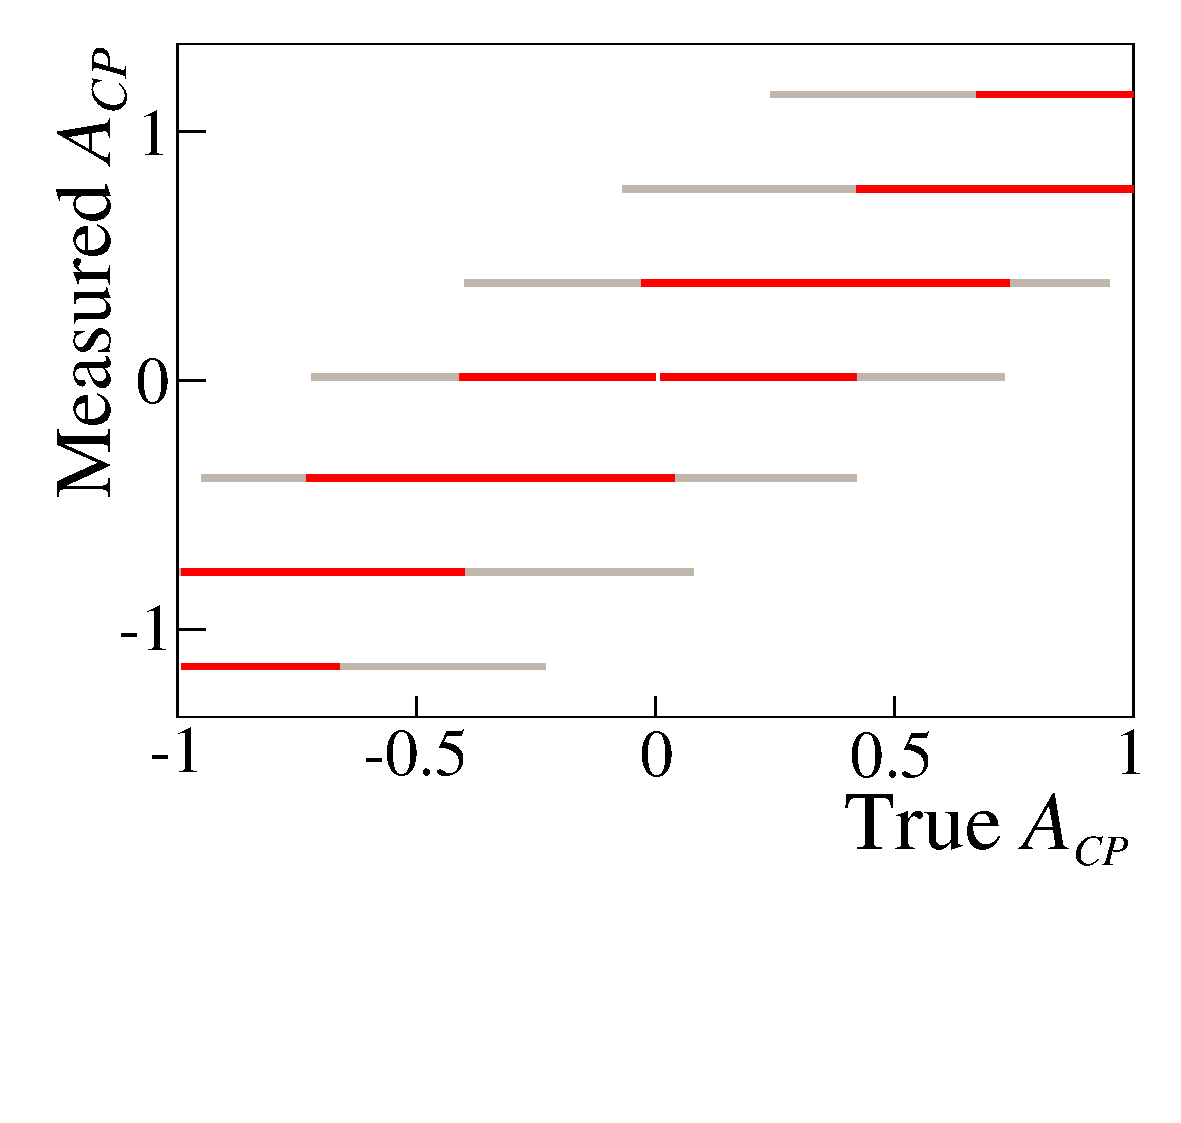
\includegraphics[width=0.48\textwidth]{fc_coverage2}
    \caption[Feldman-Cousins coverage for \acp]
    {\small
      Feldman-Cousins intervals for the \CP asymmetry, when six signal events are observed, and the
      background expectation is 0.75.
      The red stripes indicate $1\stdev$ intervals, and the grey are $2\stdev$.
    }
    \label{fig:dsphi:acp}
  \end{center}
\end{figure}

In order to find the final value of \acp, the \CP asymmetries caused by
production ($\acp^\mathrm{prod}$),
detection ($\acp^\mathrm{det}$), and
selection ($\acp^\mathrm{sel}$) must be corrected for.

The $B$ production asymmetry has been estimated by \lhcb for the decays
\decay{\Bp}{\jpsi\pip}~\cite{LHCb-PAPER-2011-024} and
\decay{\Bp}{\Dz\Kp}~\cite{LHCb-PAPER-2012-001} to be
$-(0.3\pm0.9)\pc$ and $-(0.8\pm0.7)\pc$, respectively.
For the decay \btodsphi, the only source of detection asymmetry is the pion from the \Ds decay.
This has been shown to be a very small effect, but the edges of the detector preferentially selects
one charge or the other depending on the magnet polarity.
Considering that the 2011 dataset had approximately $20\pc$ more data in one polarity than the
other, there could conceivably be an effect.
Therefore, from these values an estimate of the total $\acp^\mathrm{prod} + \acp^\mathrm{det}=-(1\pm1)\pc$
was used.
Although there are no selection requirements that preferentially select one charge or the other,
including input variables to the BDT, the selection did show a slight bias.
The selection asymmetry was given a conservative value of $(2\pm3)\pc$.

Corrections to the $\acp^\mathrm{raw}$ total to $(1\pm3)\pc$, where the error here is over a factor
of ten less than the statistical uncertainty.
Accounting for these corrections results in
\begin{align}
  \acp\big(\btodsphi\big)&=
  \acp^\mathrm{raw} - \big(\acp^\mathrm{prod} + \acp^\mathrm{det} +
  \acp^\mathrm{sel}\big)\nonumber\\
  &=
  -\big(0.01\pm0.41\stat\pm0.03\syst\big),
\end{align}
which is consistent with no observable \CPV, as expected in the SM.



